\documentclass[border=10pt]{standalone}
\usepackage[svgnames]{xcolor}
\usepackage{amsmath}
\usepackage{pgfplots}
\pgfplotsset{compat=newest}
\usepackage[sfdefault]{FiraSans}
\usepackage{FiraMono}
\renewcommand*\familydefault{\sfdefault}
\begin{document}
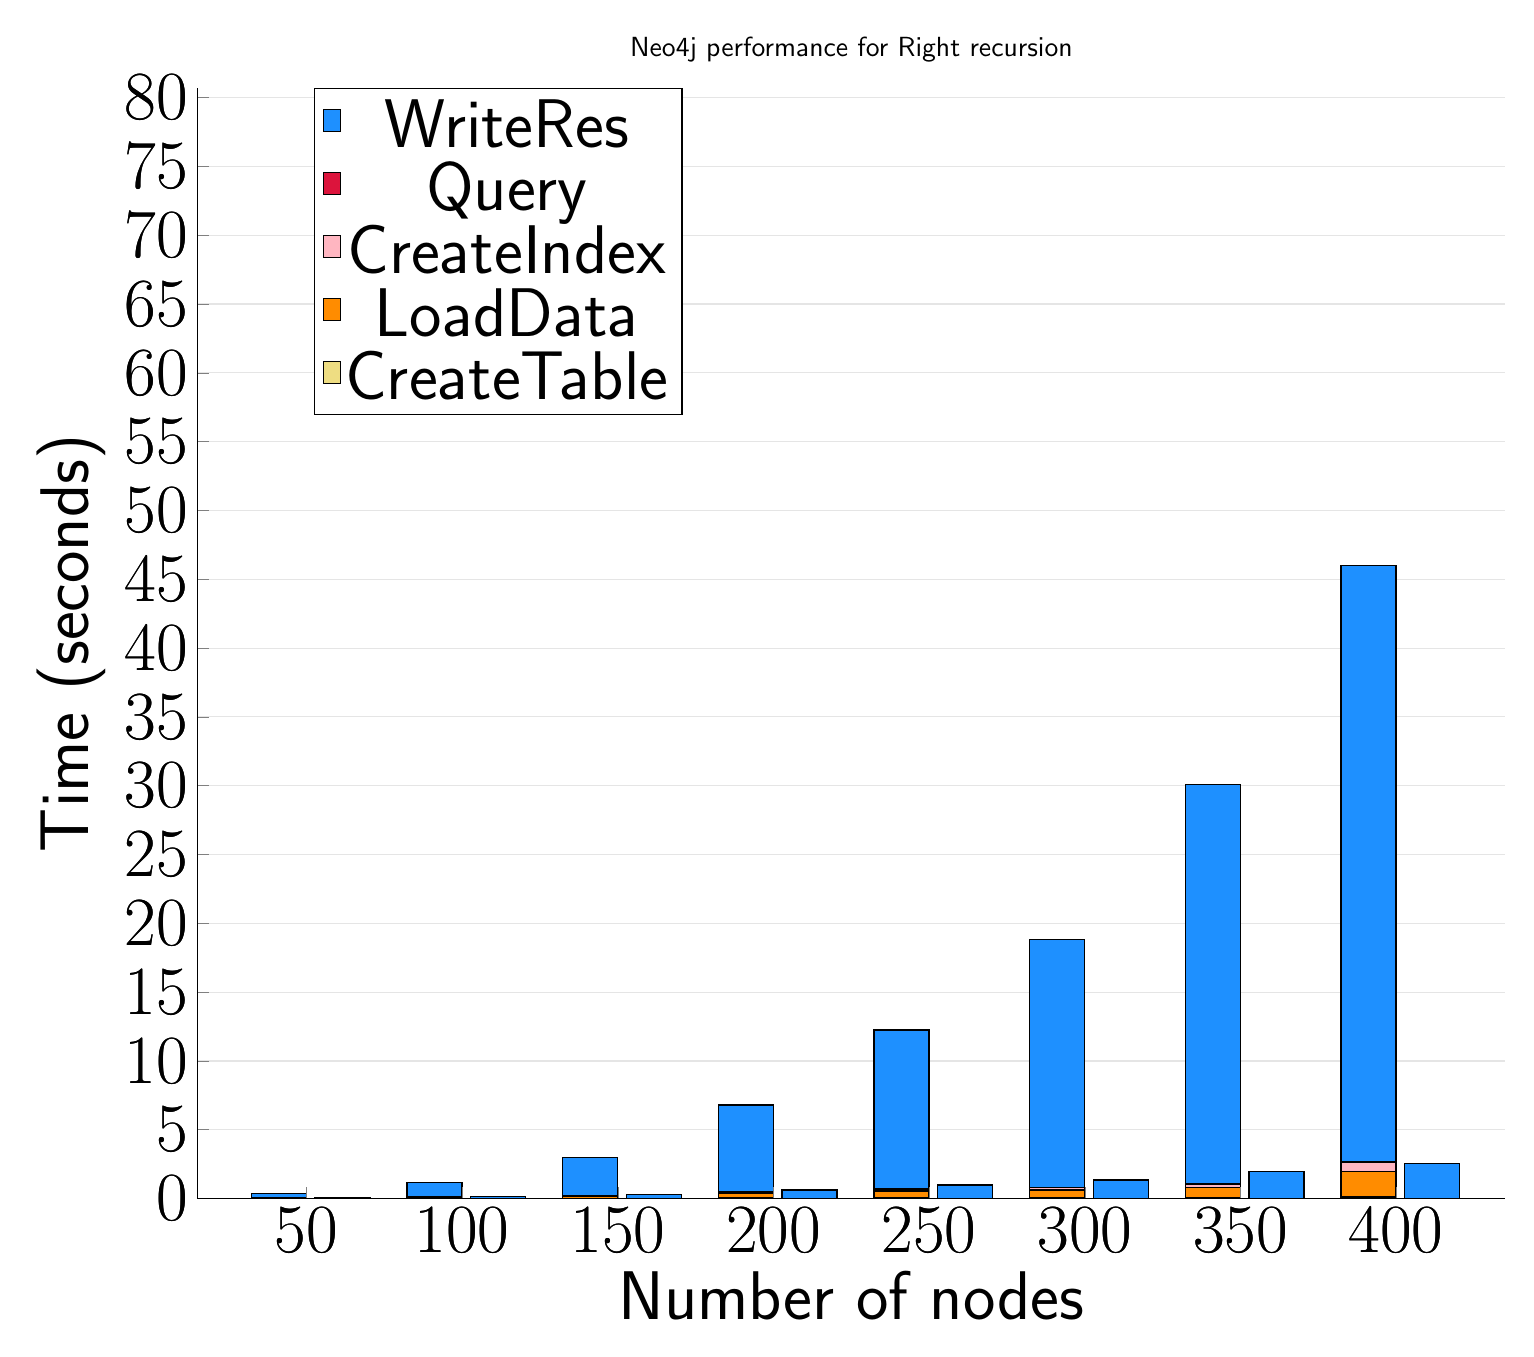
\begin{tikzpicture}
\begin{axis}[
   ybar stacked,
   title={Neo4j performance for Right recursion},
   bar shift=-10pt,
   width=1.5\textwidth,
   bar width=0.7cm,
   ymajorgrids, tick align=inside,
   major grid style={draw=gray!20},
   xtick=data,
   ymin=0, ymax=80.70666666577259,
   axis x line*=bottom,
   axis y line*=left,
   enlarge x limits=0.1,
   legend style={
       at={(0.23, 1)},
       anchor=north,
       legend columns=1,
       font=\Huge,
   },
   ylabel={Time (seconds)},
   xlabel={Number of nodes},
   label style={font=\Huge},
   tick label style={font=\Huge},
]
\addlegendimage{fill=DodgerBlue, draw=black, line width=0.2pt}
\addlegendentry{WriteRes}
\addlegendimage{fill=Crimson, draw=black, line width=0.2pt}
\addlegendentry{Query}
\addlegendimage{fill=LightPink, draw=black, line width=0.2pt}
\addlegendentry{CreateIndex}
\addlegendimage{fill=DarkOrange, draw=black, line width=0.2pt}
\addlegendentry{LoadData}
\addlegendimage{fill=LightGoldenrod, draw=black, line width=0.2pt}
\addlegendentry{CreateTable}
\addplot +[fill=LightGoldenrod, draw=black, line width=0.5pt] coordinates {
    (50, 0.013333330551783243)
    (100, 0.02333333094914754)
    (150, 0.026666663587093353)
    (200, 0.03999999910593033)
    (250, 0.05666666974623998)
    (300, 0.06666666766007741)
    (350, 0.08666666348775227)
    (400, 0.11999999980131786)
};
\addplot +[fill=DarkOrange, draw=black, line width=0.5pt] coordinates {
    (50, 0.030000001192092896)
    (100, 0.05666666726271311)
    (150, 0.11666666716337204)
    (200, 0.3333333333333333)
    (250, 0.4833333318432172)
    (300, 0.5666666651765505)
    (350, 0.7366666669646899)
    (400, 1.8400000010927517)
};
\addplot +[fill=LightPink, draw=black, line width=0.5pt] coordinates {
    (50, 0.01666666567325592)
    (100, 0.02666666607062022)
    (150, 0.043333334227403)
    (200, 0.09000000109275183)
    (250, 0.163333331545194)
    (300, 0.18000000218550363)
    (350, 0.23666666944821674)
    (400, 0.6800000021855037)
};
\addplot +[fill=Crimson, draw=black, line width=0.5pt] coordinates {
    (50, 0.019999998311201733)
    (100, 0.01666666567325592)
    (150, 0.003333332637945811)
    (200, 0.020000000794728596)
    (250, 0.0066666677594184875)
    (300, 0.003333332637945811)
    (350, 0.003333332637945811)
    (400, 0.039999996622403465)
};
\addplot +[fill=DodgerBlue, draw=black, line width=0.5pt] coordinates {
    (50, 0.2866666689515114)
    (100, 1.0399999991059303)
    (150, 2.7833333338300386)
    (200, 6.306666667262713)
    (250, 11.526666663587093)
    (300, 18.00333333512147)
    (350, 29.019999998311203)
    (400, 43.33333333581686)
};
\end{axis}
\begin{axis}[
   ybar stacked,
   bar shift=13pt,
   width=1.5\textwidth,
   bar width=0.7cm,
   ymajorgrids, tick align=inside,
   major grid style={draw=none},
   xtick=data,
   ymin=0, ymax=80.70666666577259,
   axis x line*=none,
   axis y line*=none,
   enlarge x limits=0.1,
   label style={font=\Huge},
   tick label style={font=\Huge},
]
\addplot +[fill=LightGoldenrod, draw=black, line width=0.5pt] coordinates {
    (50, 0.009999999999999986)
    (100, 0.0)
    (150, 0.003333333333333318)
    (200, 0.006666666666666654)
    (250, 0.006666666666666654)
    (300, 0.003333333333333336)
    (350, 0.003333333333333336)
    (400, 0.013333333333333343)
};
\addplot +[fill=DarkOrange, draw=black, line width=0.5pt] coordinates {
    (50, 0.0)
    (100, 0.003333333333333336)
    (150, 0.0)
    (200, 0.0)
    (250, 0.0)
    (300, 0.0033333333333333184)
    (350, 0.0)
    (400, 0.0)
};
\addplot +[fill=LightPink, draw=black, line width=0.5pt] coordinates {
    (50, 0.003333333333333318)
    (100, 0.006666666666666675)
    (150, 0.0)
    (200, 0.003333333333333337)
    (250, 0.0033333333333333184)
    (300, 0.0)
    (350, 0.006666666666666672)
    (400, 0.003333333333333336)
};
\addplot +[fill=Crimson, draw=black, line width=0.5pt] coordinates {
    (50, 0.003333333333333337)
    (100, 0.0)
    (150, 0.0)
    (200, 0.0)
    (250, 0.0)
    (300, 0.003333333333333332)
    (350, 0.0)
    (400, 0.003333333333333337)
};
\addplot +[fill=DodgerBlue, draw=black, line width=0.5pt] coordinates {
    (50, 0.03333333333333335)
    (100, 0.14)
    (150, 0.3133333333333334)
    (200, 0.6133333333333334)
    (250, 0.9700000000000001)
    (300, 1.3533333333333335)
    (350, 1.9433333333333334)
    (400, 2.5166666666666666)
};
\end{axis}
\end{tikzpicture}

\end{document}
